\documentclass{beamer}

\usepackage{alltt}%
\usetheme{Boadilla}
\usecolortheme{seahorse}

%\usepackage{listings}
\makeatletter
\def\maxwidth{ %
  \ifdim\Gin@nat@width>\linewidth
    \linewidth
  \else
    \Gin@nat@width
  \fi
}
\makeatother

\definecolor{fgcolor}{rgb}{0.345, 0.345, 0.345}
\newcommand{\hlnum}[1]{\textcolor[rgb]{0.686,0.059,0.569}{#1}}%
\newcommand{\hlstr}[1]{\textcolor[rgb]{0.192,0.494,0.8}{#1}}%
\newcommand{\hlcom}[1]{\textcolor[rgb]{0.678,0.584,0.686}{\textit{#1}}}%
\newcommand{\hlopt}[1]{\textcolor[rgb]{0,0,0}{#1}}%
\newcommand{\hlstd}[1]{\textcolor[rgb]{0.345,0.345,0.345}{#1}}%
\newcommand{\hlkwa}[1]{\textcolor[rgb]{0.161,0.373,0.58}{\textbf{#1}}}%
\newcommand{\hlkwb}[1]{\textcolor[rgb]{0.69,0.353,0.396}{#1}}%
\newcommand{\hlkwc}[1]{\textcolor[rgb]{0.333,0.667,0.333}{#1}}%
\newcommand{\hlkwd}[1]{\textcolor[rgb]{0.737,0.353,0.396}{\textbf{#1}}}%
\let\hlipl\hlkwb

\usepackage{framed}
\makeatletter
\newenvironment{kframe}{%
 \def\at@end@of@kframe{}%
 \ifinner\ifhmode%
  \def\at@end@of@kframe{\end{minipage}}%
  \begin{minipage}{\columnwidth}%
 \fi\fi%
 \def\FrameCommand##1{\hskip\@totalleftmargin \hskip-\fboxsep
 \colorbox{shadecolor}{##1}\hskip-\fboxsep
     % There is no \\@totalrightmargin, so:
     \hskip-\linewidth \hskip-\@totalleftmargin \hskip\columnwidth}%
 \MakeFramed {\advance\hsize-\width
   \@totalleftmargin\z@ \linewidth\hsize
   \@setminipage}}%
 {\par\unskip\endMakeFramed%
 \at@end@of@kframe}
\makeatother

\definecolor{shadecolor}{rgb}{.97, .97, .97}
\definecolor{messagecolor}{rgb}{0, 0, 0}
\definecolor{warningcolor}{rgb}{1, 0, 1}
\definecolor{errorcolor}{rgb}{1, 0, 0}
\newenvironment{knitrout}{}{} % an empty environment to be redefined in TeX


\usepackage[utf8]{inputenc}
\usepackage{default}

\usepackage{xcolor}%for color mixing

\usepackage{amsmath}%
\usepackage{amsfonts}%
\usepackage{amssymb}%
\usepackage{graphicx}

\usepackage{tikz}
\usepackage{multirow}
\usepackage{booktabs}

\setbeamertemplate{itemize/enumerate body begin}{\small}

%%%%%%%%%%%%%%%%%%%%%%%%%%%%%%%%%%%%%%%%%%%%%%%%%%%%%%%%%%%%%%%%%%%%%%%%%%%%%%%%%%

\title{Linear mixed models 3}
\subtitle{Random interactions and correlated random effects}
\author{Timoth\'ee Bonnet}
\date{\today}

\begin{document}

%\lstset{language=R}%code

\AtBeginSection[]
{
  \begin{frame}<beamer>
    \frametitle{}
    \tableofcontents[currentsection,sectionstyle=show/show,subsectionstyle=show/shaded/hide]% down vote\tableofcontents[currentsection,currentsubsection,hideothersubsections,sectionstyle=show/hide,subsectionstyle=show/shaded/hide] 
  \end{frame}
}

\begin{frame}{}
\centering \includegraphics[width=0.9\textwidth]{figure/ralert.jpg}
 
\end{frame}
%%%%%%%

%%%%%%%%%%%%%%%%%%%%%%%

\begin{frame}{}
\maketitle

\end{frame}
%%%%%%%%%%%%%%%%%%%%%%%


\begin{frame}{Mixed models reminder}
\centering
    \only<1>{\includegraphics[width=0.9\textwidth]{figure/graph0-1}}
    \only<2>{\includegraphics[width=0.9\textwidth]{figure/graph1-1}}
    \only<3>{\includegraphics[width=0.9\textwidth]{figure/graph2-1}}
\end{frame}
%%%%%%%%%%%
\begin{frame}{Mixed models reminder}
\vspace{-1cm}
\begin{columns}
    \begin{column}{0.5\textwidth}
     1. First model assumes residuals are independent\\
     \vspace{1cm}
     2. But they are not. Data come from five different places\\
     \vspace{1cm}
     
     3. Adding random effect ``place'' gets correct slope. Residuals are now really independent
    \end{column}

    \begin{column}{0.5\textwidth}
     \includegraphics[width=0.9\textwidth]{figure/graph0-1}\vspace{-1cm}
     \includegraphics[width=0.9\textwidth]{figure/graph1-1}\vspace{-1cm}
     \includegraphics[width=0.9\textwidth]{figure/graph2-1}
    \end{column}
\end{columns}

\end{frame}
%%%%%%%%%%%

\begin{frame}{Limitations: 1)It does not have to be parallel}
      
      \only<1>{\includegraphics[width=0.9\textwidth]{figure/graph2-1}}
      \only<2>{\includegraphics[width=0.9\textwidth]{figure/graphrslopes-1}}
 
\end{frame}
%%%%%%%%%%%

\begin{frame}{Limitations: 2)It does not have to be independent}
      
      Maybe two of the locations are very similar compare to the other ones.\\
      We assume all locations are equally different, maybe wasting information\\
      
  \centering    
      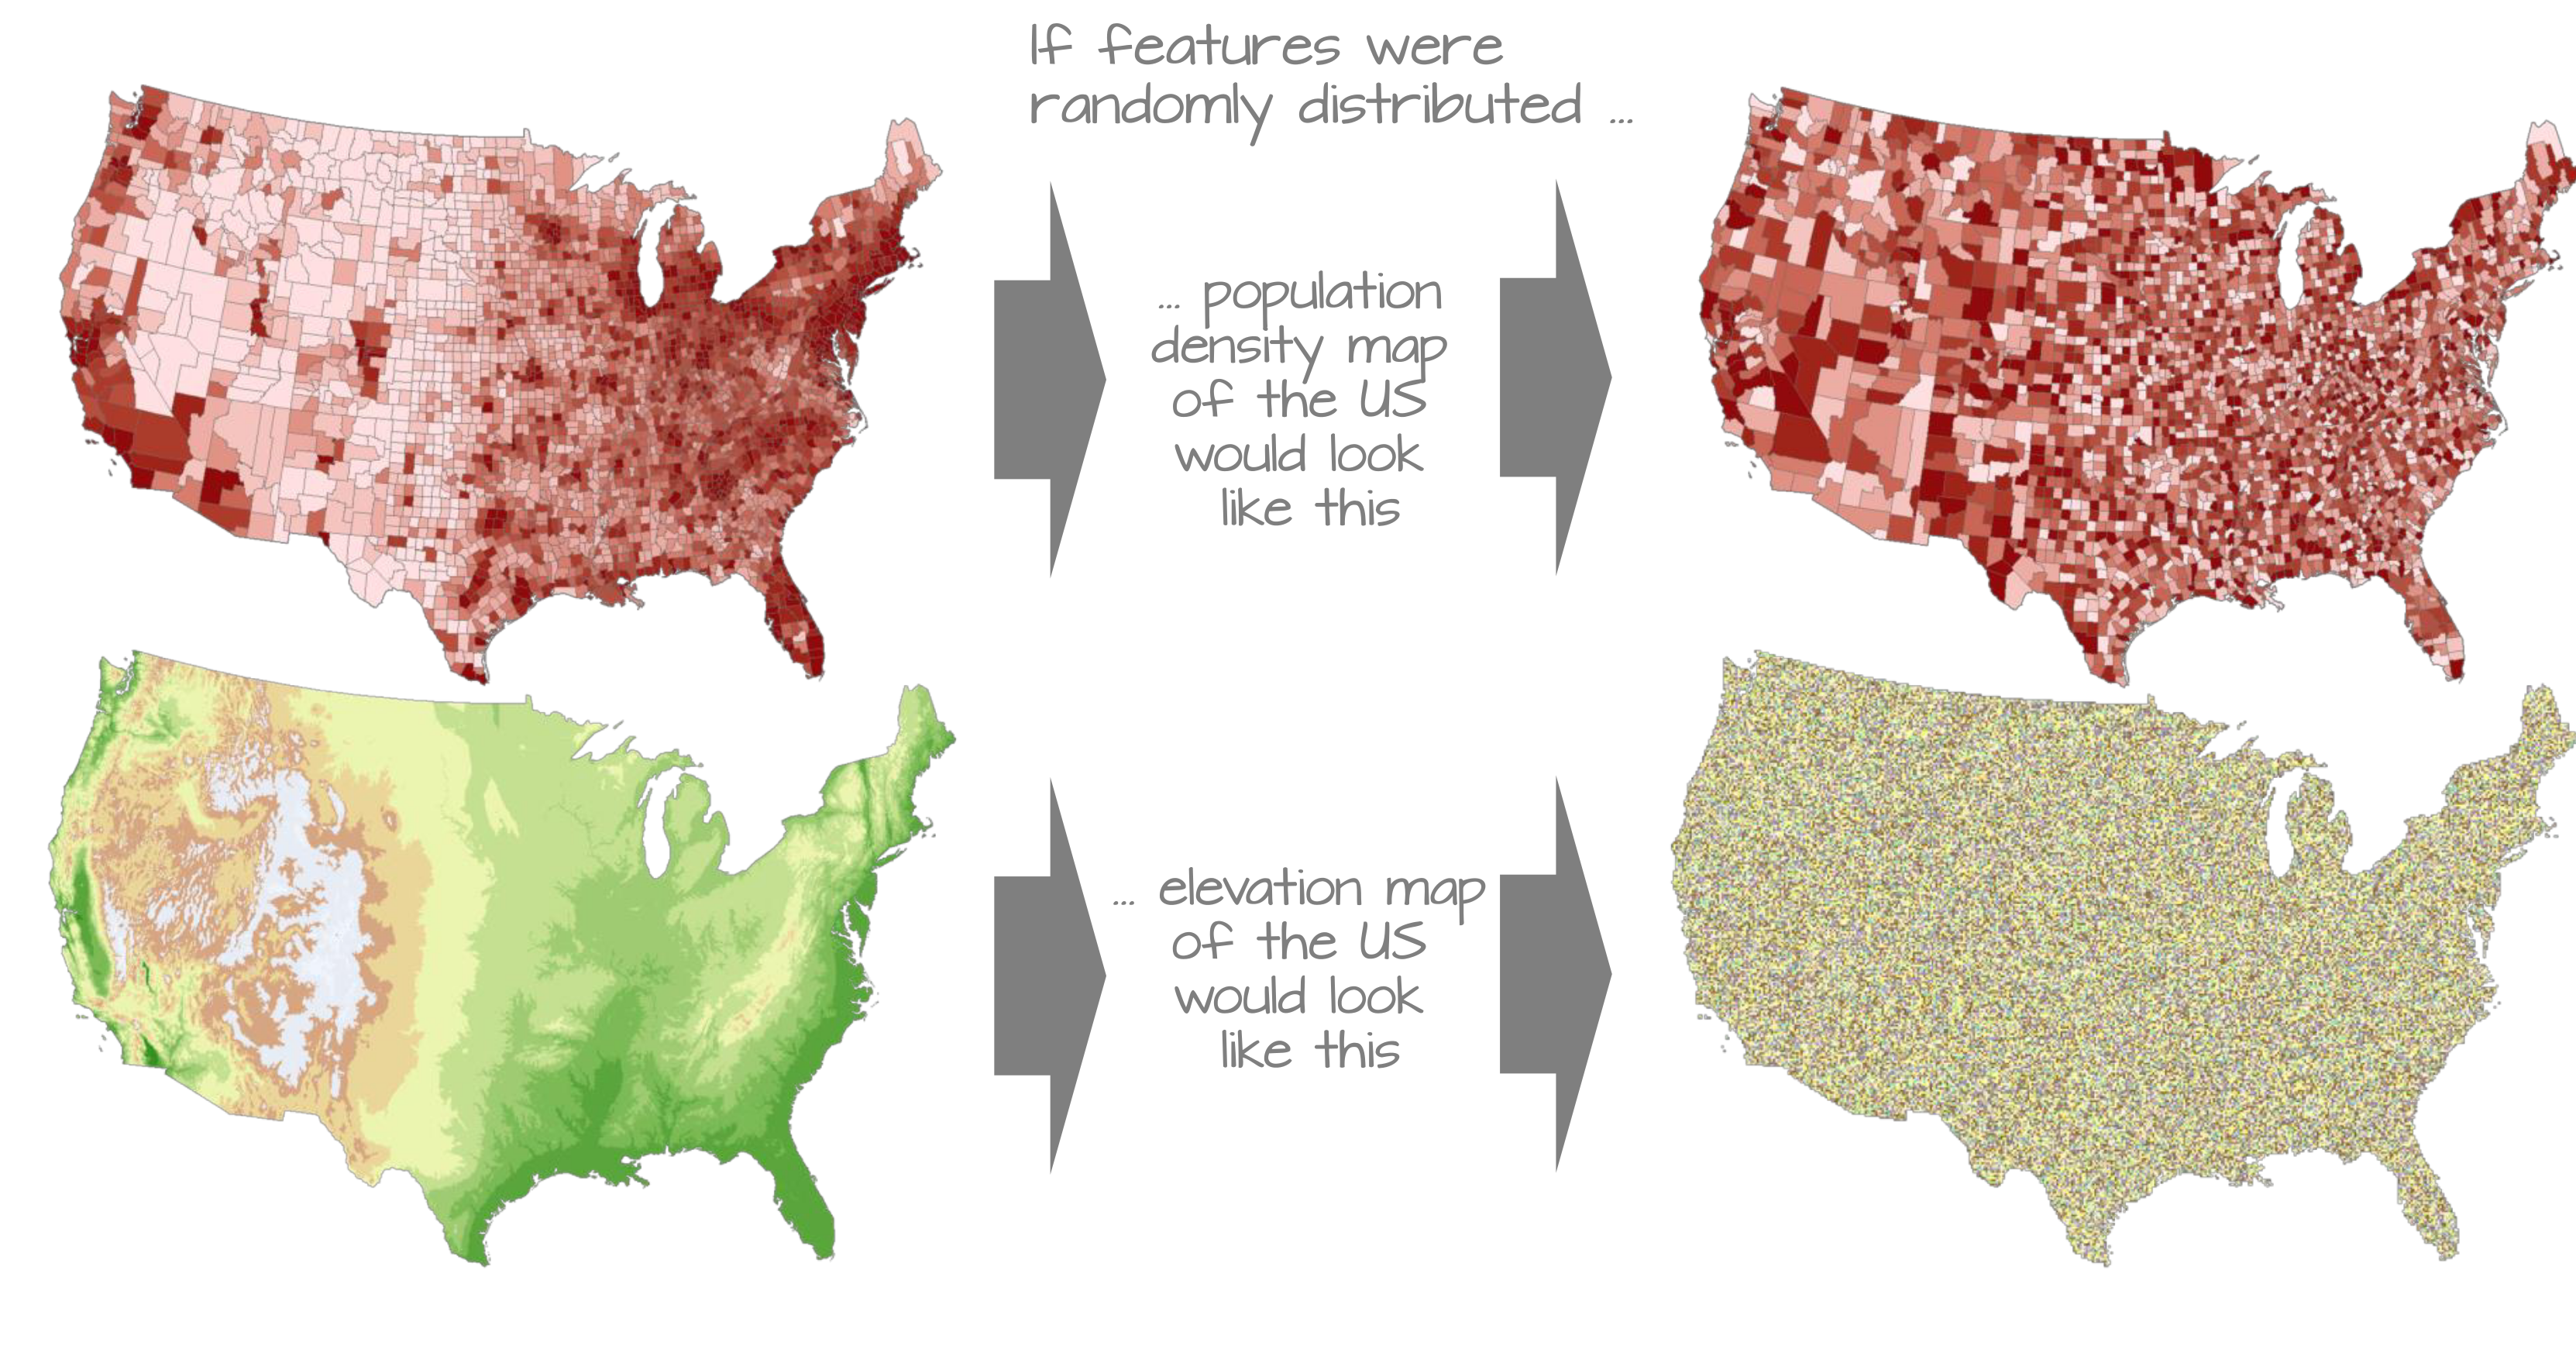
\includegraphics[width=0.8\textwidth]{figure/Random_maps.png}
      
      source: Manuel Gimond https://mgimond.github.io/Spatial/index.html
 
\end{frame}
%%%%%%%%%%%

\begin{frame}{Mixed models today}
 
 \begin{enumerate}
 \large
    \item Random interactions: \\ \textit{What if a covariate doesn't have the same effect everywhere?}
     \item Correlated random effects:\\ \textit{What if we know random effects are not independent?}
 \end{enumerate}
 

\end{frame}
%%%%%%%%%%%

\section{Beyond random intercepts}

\begin{frame}{Not only intercept vary!}
\centering
    \only<1>{
    Assume parallel slopes:
    
    \includegraphics[width=0.9\textwidth]{figure/graph2-1}}
    \only<2>{
    Allow slopes to vary:
    
    \includegraphics[width=0.9\textwidth]{figure/graphrslopes-1}}
\end{frame}
%%%%%%%

\begin{frame}{Random slopes and unbalanced data}
 We saw that random intercept could reveal a hidden pattern\\
 \textbf{What about random slopes? See exercise 1!}\\
 
 \pause
 \vfill
 \textbf{Exercise 2, visualize random slope!}\\
 \pause
\end{frame}
%%%%%%%

\begin{frame}{Application: natural selection}
 \centering
    \textbf{Exercise 3 Does natural selection vary?}
 \includegraphics[width=0.6\textwidth]{figure/cutevole}
 
\end{frame}
%%%%%%%


\begin{frame}{Random interaction with a factor}
 %the same, but think about it slightly differently
Individuals measured multiple times across two treatments
 \centering
 \includegraphics[width=0.6\textwidth]{figure/randfactor-1}
\end{frame}
%%%%%%%%

\begin{frame}{Random interaction with a factor}
 %the same, but think about it slightly differently
 Thinking about it as random intercept and random slopes
 \centering
 \includegraphics[height=0.6\textheight]{figure/reacnorm1-1}
 \includegraphics[height=0.6\textheight]{figure/reacnorm2-1}

 \texttt{lmer(y $\sim$ 1 + treat + (1 + treat|id)}
\end{frame}
%%%%%%%%

\begin{frame}{Random interaction with a factor}
 %the same, but think about it slightly differently
 Or thinking about it as two correlated traits
 \centering
 \includegraphics[height=0.6\textheight]{figure/charst1-1}
 \includegraphics[height=0.6\textheight]{figure/charst2-1}

 \texttt{lmer(y $\sim$ 1 + treat + (0 + treat|id)}\\
 \pause
 \textbf{Exercise 4!}
\end{frame}
%%%%%%%%

\begin{frame}{Beetle exercises 5, 6, 7}
 
\end{frame}
%%%%%%%%

\begin{frame}{Two sides of the random effect term}

\begin{alertblock}{\textbf{Left-hand side = what varies according to grouping}}
The \texttt{1} stands for \textbf{intercept}\\
Other things can go to the left hand side. \\
\textbf{Random interactions, random regressions, random slopes\dots}
 e.g., $y \sim 1 + x + (1 + x | something)$
\end{alertblock}
 
 \pause 
 
\begin{alertblock}{\textbf{Right-hand side = what groups observations}}
Nested, crossed et al. on the right hand side of the \texttt{|}: \texttt{(1|something)}\\
How are data related to each other, what groups them.\\
\textbf{When are the ``somethings'' correlated?}
\end{alertblock}


\end{frame}
%%%%%%%%%%%

\section{Correlated random effects}

\begin{frame}{In all models so far:}
$Response = intercept + covariate + Random + error$

$Random \sim N(0, V_{R} \mathbf{G} $)

$\mathbf{G}$ is the random effect variance covariance:
 
 \begin{center}
 \begin{tabular}[t]{cccccc}
1 & 0 & 0 & 0 & 0 & 0\\
0 & 1 & 0 & 0 & 0 & 0\\
0 & 0 & 1 & 0 & 0 & 0\\
0 & 0 & 0 & 1 & 0 & 0\\
0 & 0 & 0 & 0 & 1 & 0\\
0 & 0 & 0 & 0 & 0 & 1
 \end{tabular}
 \end{center}

 Each random effect has information only about itself.
 
\end{frame}
%%%%%%%

\begin{frame}{But one random effects can have information about others:}

\begin{center}
 \begin{tabular}[t]{cccccc}
1 & 0.5 & 0 & 0 & 0 & 0\\
0.5 & 1 & 0 & 0.25 & 0 & 0\\
0 & 0 & 1 & 0 & 0 & 0\\
0 & 0.25 & 0 & 1 & 0 & 0\\
0 & 0 & 0 & 0 & 1 & 0.9\\
0 & 0 & 0 & 0 & 0.9 & 1
 \end{tabular}
 \end{center}

 \begin{exampleblock}{For instance:}
    \begin{itemize}
     \item Spatial auto-correlation
     \item Kin in a population
     \item Related species in phylogeny
    \end{itemize}
 \end{exampleblock}

\end{frame}
%%%%%%%

\begin{frame}{Quantitative genetic demo: section 2.1}
    \begin{center}
        \includegraphics[width=0.5\textwidth]{figure/Gmatrix-1}
    \end{center}    
\end{frame}
%%%%%%%

\begin{frame}{Phylogenetic model: section 2.2}
    \begin{center}
        \includegraphics[width=0.49\textwidth]{figure/phylogeny}
        \includegraphics[width=0.49\textwidth]{figure/matphylo}
    \end{center}    
\end{frame}
%%%%%%%



\begin{frame}{Everything you need to know about mixed models}

\begin{itemize}
 \item \url{http://bbolker.github.io/mixedmodels-misc/glmmFAQ.html}
 \item Subscribe to mailing-list: \texttt{https://stat.ethz.ch/mailman/listinfo/r-sig-mixed-models}
\end{itemize}

\end{frame}
%%%%%%%%%%%%%


\end{document}
